\chapter{बिजलीघर से घर तक: प्रत्यावर्तित्र}\label{ch:g9:alternator}

पूरे साल भर के किलोवाट-घंटे तुम्हारे लेखों में से बहकर गुज़र चुके हैं
--- पर आए कहाँ से? घर से निकलती केबल के पीछे-पीछे चलो, सड़क के नीचे,
मीनारों के पार, और वह किसी विशाल हॉल में घूमती एक मशीन पर जाकर ख़त्म
होती है: \omterm{def:g9:alternator:alternator}{प्रत्यावर्तित्र}। उसका भेद इस पुस्तक की बिजली का सबसे प्यारा
अचरज है: पिछले साल वाली धारा-से-चुंबकत्व वाली खोज, उलटी चलाई हुई।

\section{प्रेरण: वही प्रभाव, उलटा}

\begin{proposition}[विद्युतचुंबकीय प्रेरण]\label{prop:g9:alternator:induction}
किसी \omterm{def:g3:first-electric-circuit:circuit}{बंद परिपथ} के पास \omterm{def:g1:magnets:magnet}{चुंबक} हिलाओ --- या \omterm{def:g1:magnets:magnet}{चुंबक} के पास परिपथ हिलाओ ---
और जब तक वह हरकत चलती है, एक \omterm{def:g8:voltage-voltmeter:voltage}{विभवांतर} उभर आता है और धारा चला देता है:
यानी बदलते चुंबकत्व से \emph{प्रेरित} हुई बिजली। मेज़ पर मिले नियम:
\begin{enumerate}
  \item प्रेरण सिर्फ़ \emph{बदलाव} करता है: कुंडली के बग़ल ठहरा हुआ
        \omterm{def:g1:magnets:magnet}{चुंबक}, तो कुछ नहीं --- \omterm{def:g1:magnets:magnet}{चुंबक} चाहे कितना ही तगड़ा हो;
  \item ज़्यादा तेज़ हरकत, ज़्यादा तगड़ा \omterm{def:g1:magnets:magnet}{चुंबक}, कुंडली के ज़्यादा
        फेरे: तो ज़्यादा बड़ा प्रेरित \omterm{def:g8:voltage-voltmeter:voltage}{विभवांतर};
  \item हरकत उलटो, प्रेरित धारा उलट जाती है --- पास आना और दूर हटना
        उलटी क़तारें चलाते हैं।
\end{enumerate}
पिछले साल धारा ने चुंबकत्व बनाया था; इस साल हिलता हुआ चुंबकत्व धारा
बनाता है। ये दोनों प्रभाव एक ही सिक्का हैं, जिसके दो पहलू पढ़े जा रहे
हैं --- और दूसरा पहलू सभ्यता को चलाता है।
\end{proposition}

\begin{method}[मेज़ पर प्रेरण]\label{met:g9:alternator:bench}
कई फेरों वाली एक कुंडली, एक छड़-चुंबक, और बीच में शून्य वाला एक
संवेदनशील उपकरण:
\begin{enumerate}
  \item उपकरण को कुंडली पर जोड़ो; और \omterm{def:g1:magnets:magnet}{चुंबक} को उसके भीतर ठहरा हुआ पकड़े
        रहो: सुई शून्य पर सोती रहती है --- अकेली ताक़त कुछ भी प्रेरित
        नहीं करती;
  \item \omterm{def:g1:magnets:magnet}{चुंबक} भीतर ठूँसो: सुई एक ओर झटका खाती है --- और हरकत रुकते ही
        उसी पल शून्य पर लौट आती है;
  \item उसे बाहर खींचो: उतना ही झटका, दूसरी ओर;
  \item ज़्यादा तेज़ ठूँसो: तो ज़्यादा बड़ा झटका। \omterm{def:g1:magnets:magnet}{चुंबक} को लय में भीतर
        और बाहर हिलाते रहो, और सुई बाएँ, दाएँ, बाएँ झूलने लगती है ---
        तुम हाथ से एक \omterm{def:g9:alternating-current:dcac}{प्रत्यावर्ती धारा} चला रहे हो।
\end{enumerate}
\end{method}

\begin{omfigure}
\begin{tikzpicture}[scale=0.85]
  \draw[thick, fill=omThm, fill opacity=0.5]
    (0.4,1.2) rectangle (2.6,2.0);
  \node[font=\small] at (1.5,1.6) {N \quad S};
  \draw[-Stealth, very thick, omExo] (2.9,1.6) -- (4.0,1.6);
  \foreach \x in {4.4,4.8,...,6.8} {
    \draw[very thick, omDef] (\x,0.9) arc (200:340:0.32 and 0.75);
  }
  \draw[thick, omDef] (4.4,0.9) -- (4.1,0.2);
  \draw[thick, omDef] (7.4,0.9) -- (7.7,0.2);
  \draw[thick] (4.1,0.2) -- (4.1,-0.4) -- (5.2,-0.4);
  \draw[thick] (7.7,0.2) -- (7.7,-0.4) -- (6.1,-0.4);
  \draw[thick, fill=white] (5.65,-0.4) circle (0.45);
  \draw[-Stealth, very thick, omThm] (5.65,-0.4) -- ++(60:0.38);
  \node[right, font=\small] at (7.9,1.6)
    {चुंबक ठूँसो: सुई झटका खाती है};
  \node[right, font=\small] at (7.9,1.0)
    {उसे ठहरा रखो: सुई सोती रहती है};
\end{tikzpicture}

{\small मेज़ पर प्रेरण: कुंडली को सिर्फ़ \emph{हिलता हुआ} \omterm{def:g1:magnets:magnet}{चुंबक} ही
जगाता है --- और सुई का झटका हरकत के साथ ही उलट जाता है।}
\end{omfigure}

\section{प्रत्यावर्तित्र}

\begin{definition}[प्रत्यावर्तित्र]\label{def:g9:alternator:alternator}
\emph{प्रत्यावर्तित्र}\index{प्रत्यावर्तित्र} प्रेरण को अथक बना देना
है: किसी ठहरी हुई कुंडली के बग़ल टिककर घुमाया गया \omterm{def:g1:magnets:magnet}{चुंबक} (या किसी
चुंबकीय क्षेत्र में घुमाई गई कुंडली)। हर आधा चक्कर एक ध्रुव को कुंडली
की ओर लाता है और फिर उसे दूर ले जाता है --- यानी बदलाव, बिना रुके
नया होता हुआ --- इसलिए प्रेरित \omterm{def:g8:voltage-voltmeter:voltage}{विभवांतर} धन, ऋण, धन झूलता रहता है:
यानी बनावट से ही \emph{प्रत्यावर्ती}, और वह ठीक वही मुलायम ज्यावक्र
खींचता है जो \omterm{met:g9:alternating-current:scope}{दोलनदर्शी} वाले अध्याय में था। हर सेकंड पचास चक्कर पर
घुमाओ और निर्गम \qty{50}{Hz} पर प्रत्यावर्तन करता है: जाल की \omterm{def:g8:sound-pitch-loudness:frequency}{आवृत्ति}
दरअसल एक घूर्णन-चाल \emph{है}, जिसे जाल का हर बिजलीघर एक ही क़दम पर
बनाए रखता है।
\end{definition}

\begin{example}[तुम्हारे पहिये पर बैठा डाइनेमो]\label{ex:g9:alternator:dynamo}
साइकिल का डाइनेमो जेब में समाता \omterm{def:g9:alternator:alternator}{प्रत्यावर्तित्र} है: पहिया किसी ठहरी
हुई कुंडली के भीतर एक नन्हा \omterm{def:g1:magnets:magnet}{चुंबक} घुमाता है, और लैंप जल उठता है ---
और जितना ज़ोर से पैडल मारो, उतना ही चमकीला तथा उतनी ही ऊँची \omterm{def:g8:sound-pitch-loudness:frequency}{आवृत्ति}
पर, ठीक जैसा मेज़ वाले नियम वादा करते हैं (और रेंगती रफ़्तार पर
टिमटिमाता हुआ, जैसा प्रत्यावर्ती वाले अध्याय ने दर्ज किया था)। और उसका
दाम भी ईमानदार है: डाइनेमो खिंचाव डालता है --- लैंप जलाने की क़ीमत
तुम्हारी टाँगों की असली मेहनत है। प्रेरण कोई \omterm{def:g5:everyday-energy:energy}{ऊर्जा} देता नहीं; वह गति
को बिजली में \emph{बदलता} है, \omterm{def:g9:kinetic-energy-safety:joule}{जूल} दर \omterm{def:g9:kinetic-energy-safety:joule}{जूल}, और उसमें से घर्षण की चुंगी
घटाकर।
\end{example}

\begin{omfigure}
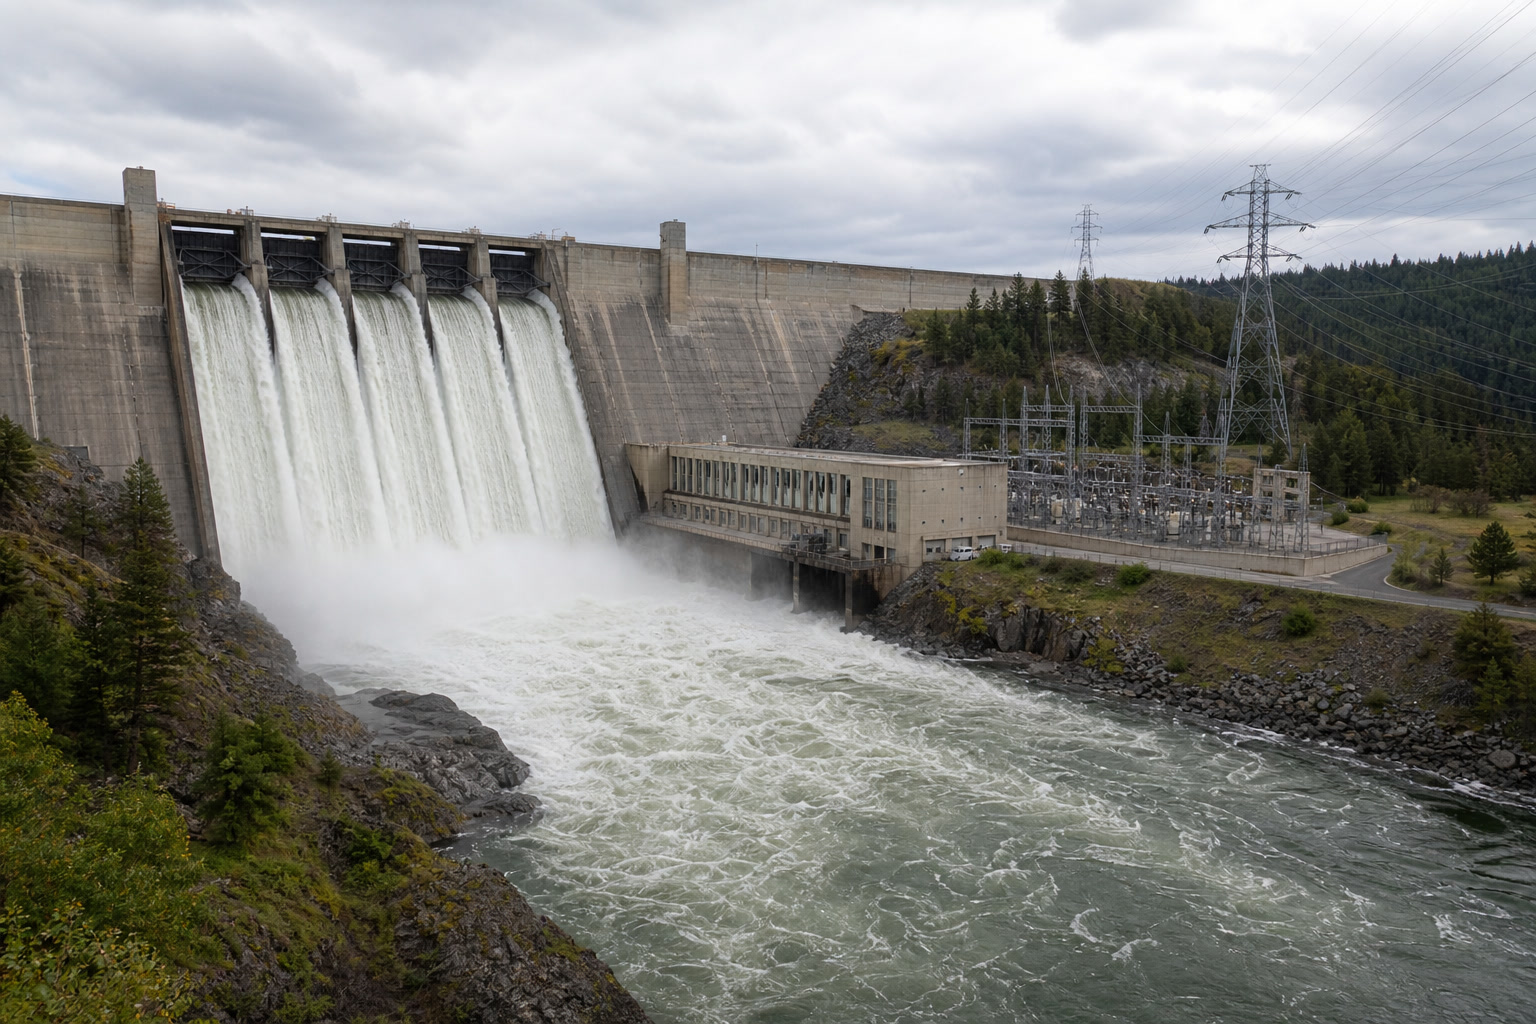
\includegraphics[width=0.55\linewidth]{images/book1/ai/g9-alternator-dam.jpg}

{\small एक जलविद्युत संयंत्र: ऊपर उठा हुआ पानी नीचे झपटता है,
टरबाइनें घुमाता है, और \omterm{def:g9:alternator:alternator}{प्रत्यावर्तित्र} उस \omterm{def:g5:everyday-energy:energy}{ऊर्जा} को तारों के साथ-साथ
दूर भेज देते हैं।}
\end{omfigure}

\section{हर बिजलीघर एक ही मशीन है}

\begin{proposition}[साझा केंद्रक]\label{prop:g9:alternator:core}
दुनिया की लगभग सारी बिजली, उसका इश्तिहार चाहे जो हो, एक ही तरीक़े से
बनती है: कोई चीज़ किसी \emph{टरबाइन} को घुमाती है --- पंखुड़ियों
वाली एक मज़बूत पवनचक्की --- और टरबाइन \omterm{def:g9:alternator:alternator}{प्रत्यावर्तित्र} को घुमाती है।
बिजलीघरों में फ़र्क़ सिर्फ़ इसका है कि \emph{पंखुड़ियों को धकेलता कौन
है}:
\begin{enumerate}
  \item तापीय संयंत्र जलते कोयले या \omterm{def:g3:solids-liquids-gases:gas}{गैस} से पानी उबालते हैं --- और भाप
        की धाराएँ टरबाइन चला देती हैं;
  \item नाभिकीय संयंत्र वही पानी परमाणु तोड़ने की \omterm{def:g5:heat-and-insulation:heat}{ऊष्मा} से उबालते हैं
        --- यानी फिर भाप;
  \item जलविद्युत बाँध किसी पहाड़ी झील को पंखुड़ियों में से गिरने देते
        हैं --- बचपन वाली बाँध की शृंखला, पूरी हुई;
  \item और \omterm{def:g2:air-around-us:wind}{पवन} टरबाइनें बिचौलिया ही हटा देती हैं: पंखुड़ियों का धक्का
        ख़ुद \omterm{def:g2:air-around-us:air}{हवा} है, और हर छत्ते में एक \omterm{def:g9:alternator:alternator}{प्रत्यावर्तित्र}।
\end{enumerate}
एक अपवाद इस नियम पर मुहर लगा देता है: सौर पट्टिकाएँ बिना किसी घुमाव के
बिजली बनाती हैं --- यानी \omterm{def:g1:light-and-shadows:source}{प्रकाश} के उस प्रभाव से, जो विश्वविद्यालय वाले
सालों का है।
\end{proposition}

\begin{omfigure}
\begin{tikzpicture}[scale=0.8]
  \node[draw, thick, omExo, font=\footnotesize, align=center,
    minimum width=2.1cm, minimum height=0.95cm] (src) at (0.9,0)
    {लपट, परमाणु,\\झील या हवा};
  \node[draw, thick, omMeth, font=\footnotesize, align=center,
    minimum width=1.9cm, minimum height=0.95cm] (tur) at (3.8,0)
    {टरबाइन\\(घुमाव!)};
  \node[draw, thick, omThm, font=\footnotesize, align=center,
    minimum width=2.0cm, minimum height=0.95cm] (alt) at (6.6,0)
    {प्रत्यावर्तित्र\\(प्रेरण)};
  \node[draw, thick, omDef, font=\footnotesize, align=center,
    minimum width=2.0cm, minimum height=0.95cm] (gri) at (9.5,0)
    {ट्रांसफ़ॉर्मर\\और जाल};
  \draw[-Stealth, very thick] (src) -- (tur);
  \draw[-Stealth, very thick] (tur) -- (alt);
  \draw[-Stealth, very thick] (alt) -- (gri);
  \node[below, font=\footnotesize] at (2.35,-0.75) {ऊष्मा या गति};
  \node[below, font=\footnotesize] at (5.2,-0.75) {घूर्णन};
  \node[below, font=\footnotesize] at (8.05,-0.75)
    {प्रत्यावर्ती धारा};
\end{tikzpicture}

{\small हर संयंत्र, एक ही शृंखला: कोई चीज़ टरबाइन घुमाती है, टरबाइन
\omterm{def:g9:alternator:alternator}{प्रत्यावर्तित्र} घुमाती है, और बाक़ी काम प्रेरण कर देता है। संयंत्र दर
संयंत्र सिर्फ़ पहला डिब्बा बदलता है।}
\end{omfigure}

\begin{example}[शृंखलाओं का लेखा]\label{ex:g9:alternator:chains}
हर संयंत्र को बचपन वाली ऊर्जा-शृंखला की तरह लिखो, पर अब पेशेवर शब्दों
के साथ। बाँध: जमा की हुई ऊँचाई $\to$ गिरते पानी की गति $\to$ घूर्णन
$\to$ बिजली --- और याद रखो कि उस झील को सूर्य ने वाष्पीकरण से उठाया
था: जलविद्युत दरअसल बारिश में टली हुई धूप है। कोयले का संयंत्र:
रासायनिक भंडार $\to$ \omterm{def:g5:heat-and-insulation:heat}{ऊष्मा} $\to$ भाप की गति $\to$ घूर्णन $\to$ बिजली
--- और हर तीर पर गरमाहट रिसती हुई, जैसा ठंडा करने वाली मीनारों के
गुबार क़बूल कर लेते हैं। \omterm{def:g2:air-around-us:air}{हवा}: चलती हुई \omterm{def:g2:air-around-us:air}{हवा} (जिसे सूर्य ने हिलाया) सीधे
घूर्णन तक। जिन स्रोतों को क़ुदरत दोबारा भर देती है --- पानी, \omterm{def:g2:air-around-us:air}{हवा}, धूप
--- उन्हें \emph{नवीकरणीय}\index{नवीकरणीय} कहते हैं; जबकि जलाए और तोड़े
गए भंडार इंसानी पैमानों पर हमेशा के लिए ख़र्च हो जाते हैं।
\end{example}

\begin{remark}[मीनारें चार लाख वोल्ट पर क्यों गुनगुनाती हैं]\label{rem:g9:alternator:transport}
प्रत्यावर्ती वाले अध्याय का आख़िरी वादा चुकता होता है। मान लो किसी
क़स्बे को दस करोड़ \omterm{def:g9:electric-power-energy:power}{वाट} चाहिए। $P = U I$ के हिसाब से वह \omterm{def:g9:electric-power-energy:power}{शक्ति} सधे हुए
\omterm{def:g8:voltage-voltmeter:voltage}{विभवांतर} पर विशाल धारा बनकर सफ़र कर सकती है --- या विशाल \omterm{def:g8:voltage-voltmeter:voltage}{विभवांतर} पर
सधी हुई धारा बनकर। पर तार \emph{धारा} से गरम होते हैं (यानी वही पुराना
\omterm{prop:g8:electric-current-effects:three}{ऊष्मीय प्रभाव}), और मीनारों के गरम होने का हर अंश चुकाई हुई \omterm{def:g5:everyday-energy:energy}{ऊर्जा} है जो
कौवों के हवाले हो जाती है। इसलिए जाल साँस रोक देने वाले विभवांतरों पर
ढोता है --- लाखों \omterm{def:g8:voltage-voltmeter:voltage}{वोल्ट}, नन्ही धाराएँ, और कम से कम नुक़सान --- और फिर
मोहल्ले दर मोहल्ले \omterm{def:g8:voltage-voltmeter:voltage}{विभवांतर} उतारकर तुम्हारी दीवार की सधी हुई
\qty{230}{V} तक ले आता है। उतारने वाली वह मशीन, यानी
\emph{ट्रांसफ़ॉर्मर}, दो कुंडलियाँ और एक बार फिर वही प्रेरण है --- और
वह सिर्फ़ प्रत्यावर्तन करती धारा पर ही काम करती है: पूरा जाल AC इसलिए
बोलता है कि ट्रांसफ़ॉर्मर वही बोलता है।
\end{remark}

\section{अभ्यास}

\begin{exercise}[$\star$]\label{exo:g9:alternator:1}
प्रेरण के तीनों मेज़ वाले नियम बताओ। \emph{ठहरा हुआ} तगड़ा \omterm{def:g1:magnets:magnet}{चुंबक} क्या
प्रेरित करता है?
\end{exercise}

\begin{exercise}[$\star$]\label{exo:g9:alternator:2}
\omterm{def:g9:alternator:alternator}{प्रत्यावर्तित्र} का निर्गम प्रत्यावर्तन क्यों करता है? चिह्न के बदलावों
को घूर्णन से जोड़ो।
\end{exercise}

\begin{exercise}[$\star$]\label{exo:g9:alternator:3}
कोई \omterm{def:g9:alternator:alternator}{प्रत्यावर्तित्र} किस घूर्णन-चाल पर \qty{50}{Hz} वाले जाल को खिलाता
है? और इसलिए जाल के हर बिजलीघर को किस बात पर सहमत होना ही पड़ता है?
\end{exercise}

\begin{exercise}[$\star$]\label{exo:g9:alternator:4}
हर बिजलीघर के दोनों सार्वत्रिक डिब्बों के नाम बताओ, और वह अकेला डिब्बा
भी जो कोयले, परमाणु, बाँध और \omterm{def:g2:air-around-us:air}{हवा} के बीच बदलता है।
\end{exercise}

\begin{exercise}[$\star$]\label{exo:g9:alternator:5}
पहाड़ी झील से तुम्हारे लैंप तक जलविद्युत की शृंखला लिखो --- और उस
आकाशीय मशीन का नाम भी बताओ जिसने वह झील भरी।
\end{exercise}

\begin{exercise}[$\star$]\label{exo:g9:alternator:6}
डाइनेमो का लैंप चालू होते ही पैडल मारना उसी पल भारी क्यों हो जाता है?
कौन-सा सिद्धांत इसे और किसी तरह होने से मना कर देता है?
\end{exercise}

\begin{exercise}[$\star$]\label{exo:g9:alternator:7}
\omterm{ex:g9:alternator:chains}{नवीकरणीय} और ग़ैर-नवीकरणीय में छाँटो: \omterm{def:g2:air-around-us:air}{हवा}; कोयला; बाँध की झील; यूरेनियम;
धूप। यह छँटाई किस बात से तय होती है?
\end{exercise}

\begin{exercise}[$\star$]\label{exo:g9:alternator:8}
जाल अपनी \omterm{def:g9:electric-power-energy:power}{शक्ति} लाखों \omterm{def:g8:voltage-voltmeter:voltage}{वोल्ट} पर क्यों ढोता है? वह सूत्र बताओ जो यह चुनाव
देता है, और वह प्रभाव भी जो फ़ैसला करता है।
\end{exercise}

\begin{exercise}[$\star\star$]\label{exo:g9:alternator:9}
प्रदर्शन वाला \omterm{def:g9:alternator:alternator}{प्रत्यावर्तित्र} धीरे-धीरे हाथ से घुमाने पर अपना लैंप
मद्धम और साफ़ टिमटिमाहट के साथ जलाता है; और तेज़ घुमाने पर चमकीला तथा
टिका हुआ। दोनों बदलाव मेज़ वाले नियमों और \omterm{def:g8:sound-pitch-loudness:frequency}{आवृत्ति} वाले अध्याय से
समझाओ।
\end{exercise}

\begin{exercise}[$\star\star$]\label{exo:g9:alternator:10}
कोई संयंत्र \qty{1e8}{W} पहुँचाता है। \qty{230}{V} पर और
\qty{400000}{V} पर ज़रूरी धाराओं की तुलना करो (वैज्ञानिक संकेतन में)।
इनमें से कौन-सी धारा असली केबल ढो सकती थीं?
\end{exercise}

\begin{exercise}[$\star\star$]\label{exo:g9:alternator:11}
तापीय और नाभिकीय संयंत्र, दिल से, विस्तृत केतलियाँ ही हैं। इस नारे का
बचाव उनकी शृंखलाओं से करो --- और वह अकेली कड़ी ढूँढ़ो जहाँ दोनों अलग
होती हैं।
\end{exercise}

\begin{exercise}[$\star\star\star$]\label{exo:g9:alternator:12}
वह भव्य सैर, उलटी चलाई हुई: आज रात तुम्हारा लैंप \qty{230}{V} पर दमक
रहा है। उसकी \omterm{def:g5:everyday-energy:energy}{ऊर्जा} को हर डिब्बे से होते हुए उलटी दिशा में खींचो ---
ट्रांसफ़ॉर्मर, मीनारें, \omterm{def:g9:alternator:alternator}{प्रत्यावर्तित्र}, टरबाइन, और अपनी पसंद का एक
प्राथमिक भंडार --- और हर पड़ाव पर \omterm{def:g5:everyday-energy:energy}{ऊर्जा} का रूप तथा रास्ते के रिसाव भी
बताओ। फिर बचपन वाले सवाल का जवाब नौवीं \omterm{def:g6:sun-earth-moon:axisorbit}{कक्षा} के एक वाक्य में दो:
तुम्हारे कमरे का \omterm{def:g1:light-and-shadows:source}{प्रकाश} आख़िरकार आता कहाँ से है?
\end{exercise}

\section{समस्या: बिजलीघर में रात की पाली}

\begin{problem}[{सप्ताहांत समस्या --- जलविद्युत बिजलीघर में रात की
पाली; प्रेरण, एक क़दम पर चलना और तूफ़ान; अभियंता की
बही}]\label{pb:g9:alternator:1}
तुम घाटी के बाँध पर रात के अभियंता के साथ-साथ चल रहे हो --- ऊपर झील,
नीचे क़स्बा, और बीच में गुनगुनाते \omterm{def:g9:alternator:alternator}{प्रत्यावर्तित्र}।

\medskip\noindent\textbf{भाग I --- मशीन-हॉल।}
\begin{enumerate}
  \item अभियंता एक फाटक खोलती हैं: पानी तीसरी टरबाइन में से गरजता है,
        और उसके \omterm{def:g9:alternator:alternator}{प्रत्यावर्तित्र} के उपकरण जाग उठते हैं। झील से बसबार तक
        की ऊर्जा-शृंखला लिखो।
  \item \omterm{def:g9:alternator:alternator}{प्रत्यावर्तित्र} के भीतर क्या हिलता है और क्या ठहरा रहता है ---
        और कुछ हिलना ज़रूरी ही क्यों है?
  \item जाल \qty{50}{Hz} पर चलता है। अभियंता एक सुई-पट्टी पर नज़र
        रखती हैं जो तीसरी टरबाइन को ठीक मेल खाते घूर्णन पर बनाए रखती
        है। ग़लत \omterm{def:g7:motion-average-speed:formula}{चाल} पर क्या बिगड़ जाता है? (उसके \omterm{def:g8:voltage-voltmeter:voltage}{विभवांतर} की \omterm{def:g8:sound-pitch-loudness:frequency}{आवृत्ति}
        क्या करती?)
  \item एक प्रशिक्षु पूछता है कि क्या घूर्णक में ज़्यादा तगड़ा \omterm{def:g1:magnets:magnet}{चुंबक}
        ``मुफ़्त'' फ़ालतू \omterm{def:g9:electric-power-energy:power}{शक्ति} दे देगा। डाइनेमो की ईमानदार क़ीमत से
        उस सपने को सुधारो।
\end{enumerate}

\medskip\noindent\textbf{भाग II --- क़स्बे की माँग।}
\begin{enumerate}[resume]
  \item 03:00 पर क़स्बा \qty{2e7}{W} खींच रहा है। ढोने वाली लाइन के
        \qty{200000}{V} पर बिजलीघर से कितनी धारा निकलती है?
  \item वही \omterm{def:g9:electric-power-energy:power}{शक्ति} \qty{230}{V} पर कितनी धारा माँगती --- और यह तुलना
        ट्रांसफ़ॉर्मर के काम के बारे में क्या कहती है?
  \item 07:00 पर केतलियाँ और हीटर जागते हैं: माँग दोगुनी हो जाती है।
        अभियंता को टरबाइनों को किस चीज़ का ज़्यादा खिलाना पड़ेगा, और
        कम खिलाने पर जाल की \omterm{def:g8:sound-pitch-loudness:frequency}{आवृत्ति} का क्या होता? (बोझ पड़ने पर
        मशीनें धीमी पड़ती हैं, ठीक चढ़ाई पर चढ़ते साइकिल सवार की
        तरह।)
  \item बिजलीघर की बहन इकाई --- पहाड़ी पर लगा पवन-खेत --- \omterm{def:g2:air-around-us:air}{हवा} थमते ही
        बाहर हो जाती है। उसकी शृंखला का कौन-सा डिब्बा नाकाम हुआ, और
        कौन-से डिब्बे पूरी तरह भले-चंगे खड़े रहे?
\end{enumerate}

\medskip\noindent\textbf{भाग III --- तूफ़ान।}
\begin{enumerate}[resume]
  \item बिजली गिरने से एक ढोने वाली लाइन कट जाती है; विच्छेदक चल
        पड़ते हैं। अभियंता \omterm{def:g9:electric-power-energy:power}{शक्ति} को पड़ोसी लाइनों से घुमा देती हैं।
        जाल का कौन-सा गुण --- एक विशाल समांतर जाल होना --- यह
        घुमाव मुमकिन बनाता है?
  \item इस भागदौड़ में किसी गोदाम की बत्तियाँ एक मिनट के लिए भूरी-सी
        मंद पड़ जाती हैं। इसका मतलब निकालो: क्या ढल गया, और गोदाम की
        मोटरें तथा लैंप थोड़ी देर के लिए किस चीज़ के भूखे रह गए?
  \item भोर: बही में प्रशिक्षुओं को यह समझाना है कि पूरी रात की बिजली
        अपने उद्गम पर धूप ही थी। दो पंक्तियों वाली वह व्याख्या लिखो
        (झील, वाष्पीकरण, बारिश)।
  \item बही की आख़िरी पंक्ति, रिवाज के मुताबिक़: रात की भौतिकी एक वाक्य
        में --- और उसमें गति, चुंबकत्व तथा क़स्बे की सुबह वाली केतली,
        तीनों।
\end{enumerate}
\end{problem}
